\section{\system{}: Evaluation}
Using the \system{} implementation, we evaluate the system on it's ability to avoid a given country, performance, and scalability in terms of storage and costs.

\subsection{Country Avoidance}
As the primary goal of the system is to provide country avoidance for a given 
country, we measured how much avoidance the system achieves.  We did so by first 
calculating the number of {\it default} paths that avoid a given country.  Then 
we added a single relay, and calculated how many domains the client could 
access without traversing through the given country.  This was repeated for 
the remaining two relays.  The evaluation was conducted under the condition that 
the client wished to avoid the United States when accessing the Netherlands top 
100 domains, and the results are shown in Figure \ref{fig:avoidance_eval}.

\begin{figure}[b!]
\centering
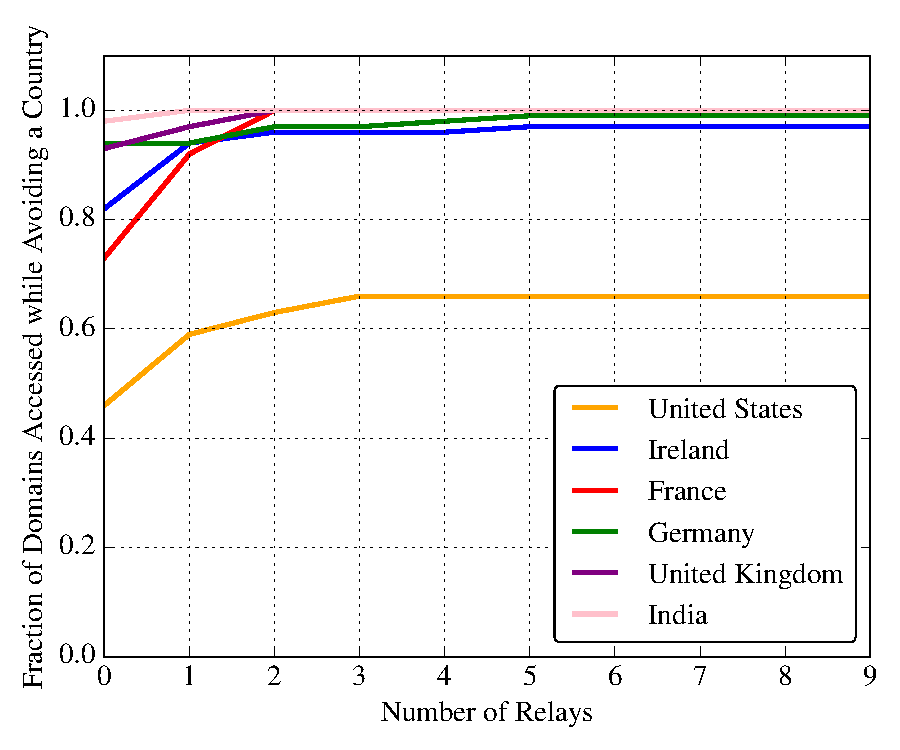
\includegraphics[width=.5\textwidth]{avoidance_n_relays}
\caption{How much avoidance different numbers and locations of relays achieve.}
\label{fig:avoidance_eval}
\end{figure}

It is evident that \system{} helps a client avoid a foreign country (in this case 
the United States), as the fraction of domains accessible without traversing 
the United States without \system{} is .46 and with \system{} is .63.  Additionally, 
it is clear that adding the first relay provides the greatest increase in 
provided avoidance, while subsequent relays provide a significantly 
smaller amount (or no) additional avoidance.

\subsection{Performance}
A system is not usable if the performance is significantly worse than what a user
is accustomed to.  To measure the performance of \system{}, we {\tt wget} each 
of the top 100 domains from the client machine in the Netherlands, while 
using the PAC file.  Based on the {\tt wget} output, we calculate the number 
of seconds to access content using our system. Figure \ref{fig:latency} shows 
the time to access content with \system{} in comparison to the time to access the 
same content without \system{} (using default paths).  

\begin{figure}[t]
\centering
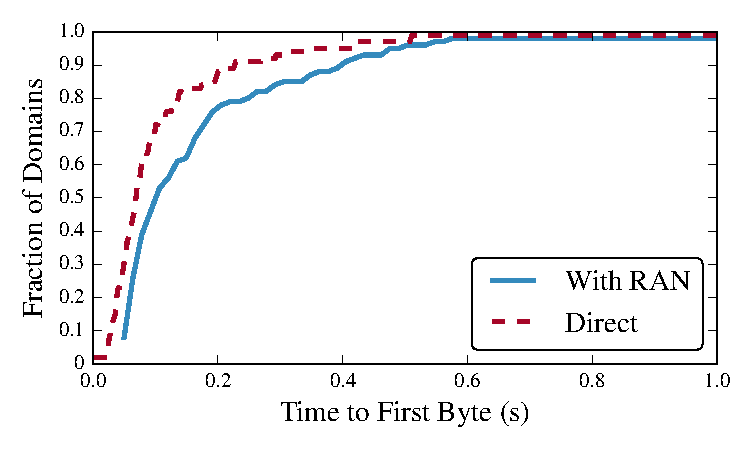
\includegraphics[width=.5\textwidth]{latency}
\caption{Latency difference when accessing a webpage via \system{} vs. default paths. 
The difference is calculated by \system{} latency minus default latency, and represents 
the additional latency cost of our system.}
\label{fig:latency}
\end{figure}

We can see that the performance of \system{} is not significantly worse than that 
of default paths.  In fact, in some cases the performance of \system{} is {\it 
better} than that of default paths.  This could be a result of the relays 
keeping local traffic local, or due to a closer content replica being selected. 
These results show that \system{}'s performance is comparable to the performance 
of accessing domains without \system{}.

\subsection{Storage}
As the number of clients increase, and subsequently the number of paths being 
computed increases, the amount of storage must remain reasonable.  The storage 
used by paths can be calculated:

\[Storage(D,R) = (D x R) + 2(C x R) + (C x D) \]

D is the number of domains; R is the number of relays; C is the number of 
clients.  For the prototype with a single client, the storage space for all 
paths computed is 480KB.  As there is a single PAC file for all clients in 
a country, C will grow much slower than if there was a different PAC file for 
each individual client.  There are 196 countries in the world today, and if 
paths and a PAC file were generated for each country, with 100 domains, and 
three relays, the storage would only be 94MB.  This provides plenty of storage 
for increasing the number of domains included in the PAC file or increasing 
the number of relays in the system.

\subsection{Costs}
In addition to storage, the cost of the measurements used in the system must 
be taken into account.  RIPE Atlas credits are a limited resource, and therefore 
we must earn more credits than we are spending on measurements.  The cost 
in credits follows the equation:

\[Credit\_Cost(D,R,C) = 60(C x R) + 60(C x D)\]

The prototype cost 6,180 credits, but because these paths are updated each hour, then 
the daily credit cost is 148,320 credits.  In return for hosting a RIPE Atlas 
probe, we earn 216,000 credits per day, which will support our existing 
prototype.  In order to provide for more clients, more domains, or more 
resources, we can tune the system to re-compute paths less frequently (only when necessary).
